\section*{Unterteilung der Galaxie in Zellen}

Um den Rechenaufwand, der bei der Berechnung der wirkenden Kräfte entsteht,
zu minimieren, wird die Galaxie in verschiedene Zellen unterteilt:

\begin{center}\vspace{1cm}
\includegraphics[width=0.8\linewidth]{figs/cells_2D}
\label{fig:galaxy_cells}
\end{center}

\begin{center}
\includegraphics[width=1\linewidth]{figs/cells}
\label{fig:galaxy_cells_3d}
\end{center}\vspace{-3cm}
